\documentclass[11pt,a4paper]{article}
\usepackage[textwidth=37em,vmargin=30mm]{geometry}
\usepackage{calc,xunicode,amsmath,amssymb,paralist,enumitem,tabu,booktabs,datetime2,xeCJK,xeCJKfntef,listings}
\usepackage{tocloft,fancyhdr,tcolorbox,xcolor,graphicx,eso-pic}

\usepackage[hidelinks]{hyperref}
\hypersetup{
    colorlinks=false,
    pdfpagemode=FullScreen,
    pdftitle={Web Digest - DATESTRING}
}

\setdefaultleftmargin{2em}{2em}{1em}{1em}{1em}{1em}

\usepackage{xeCJK,xeCJKfntef}
\newcommand{\myvphantom}[0]{\vphantom{QWERTYUIOPASDFGHJKLZXCVBNMqwertyuiopasdfghjklzxcvbnm1234567890ςρθδφγηξλζχψβμ\"A}}
\xeCJKsetup{PunctStyle=plain,RubberPunctSkip=false,CJKglue=\myvphantom\hskip 0pt plus 0.1em minus 0.05em,CJKecglue=\myvphantom\hskip 0.22em plus 200pt}
\XeTeXlinebreaklocale "zh"
\XeTeXlinebreakskip = 0pt


\setmainfont[Numbers=Lining]{Brygada 1918}
\setromanfont[Numbers=Lining]{Brygada 1918}
\setsansfont[Numbers=Lining]{IBM Plex Sans}
\setmonofont{JetBrains Mono NL}
\setCJKmainfont{Noto Serif CJK SC}
\setCJKromanfont{Noto Serif CJK SC}
\setCJKsansfont{Noto Sans CJK SC}
\setCJKmonofont{Noto Sans CJK SC}

\setlength{\parindent}{0pt}
\setlength{\parskip}{8pt}
\linespread{1.15}

\lstset{
	basicstyle=\ttfamily\footnotesize,
	numbersep=5pt,
	backgroundcolor=\color{black!5},
	showspaces=false,
	showstringspaces=false,
	showtabs=false,
	tabsize=2,
	captionpos=b,
	breaklines=true,
	breakatwhitespace=true,
	breakautoindent=true,
	linewidth=\textwidth
}






\newcommand{\coverpic}[2]{
    % argv: itemurl, authorname
    Cover photo by #2~~~~(\href{#1}{#1})
}
\newcommand{\makeheader}[0]{
    \begin{center}
        
        \rmfamily\scshape
        \fontsize{62pt}{70pt}\selectfont
        WEB\hfill DIGEST
        
        \vfill
        % \vskip 30pt
        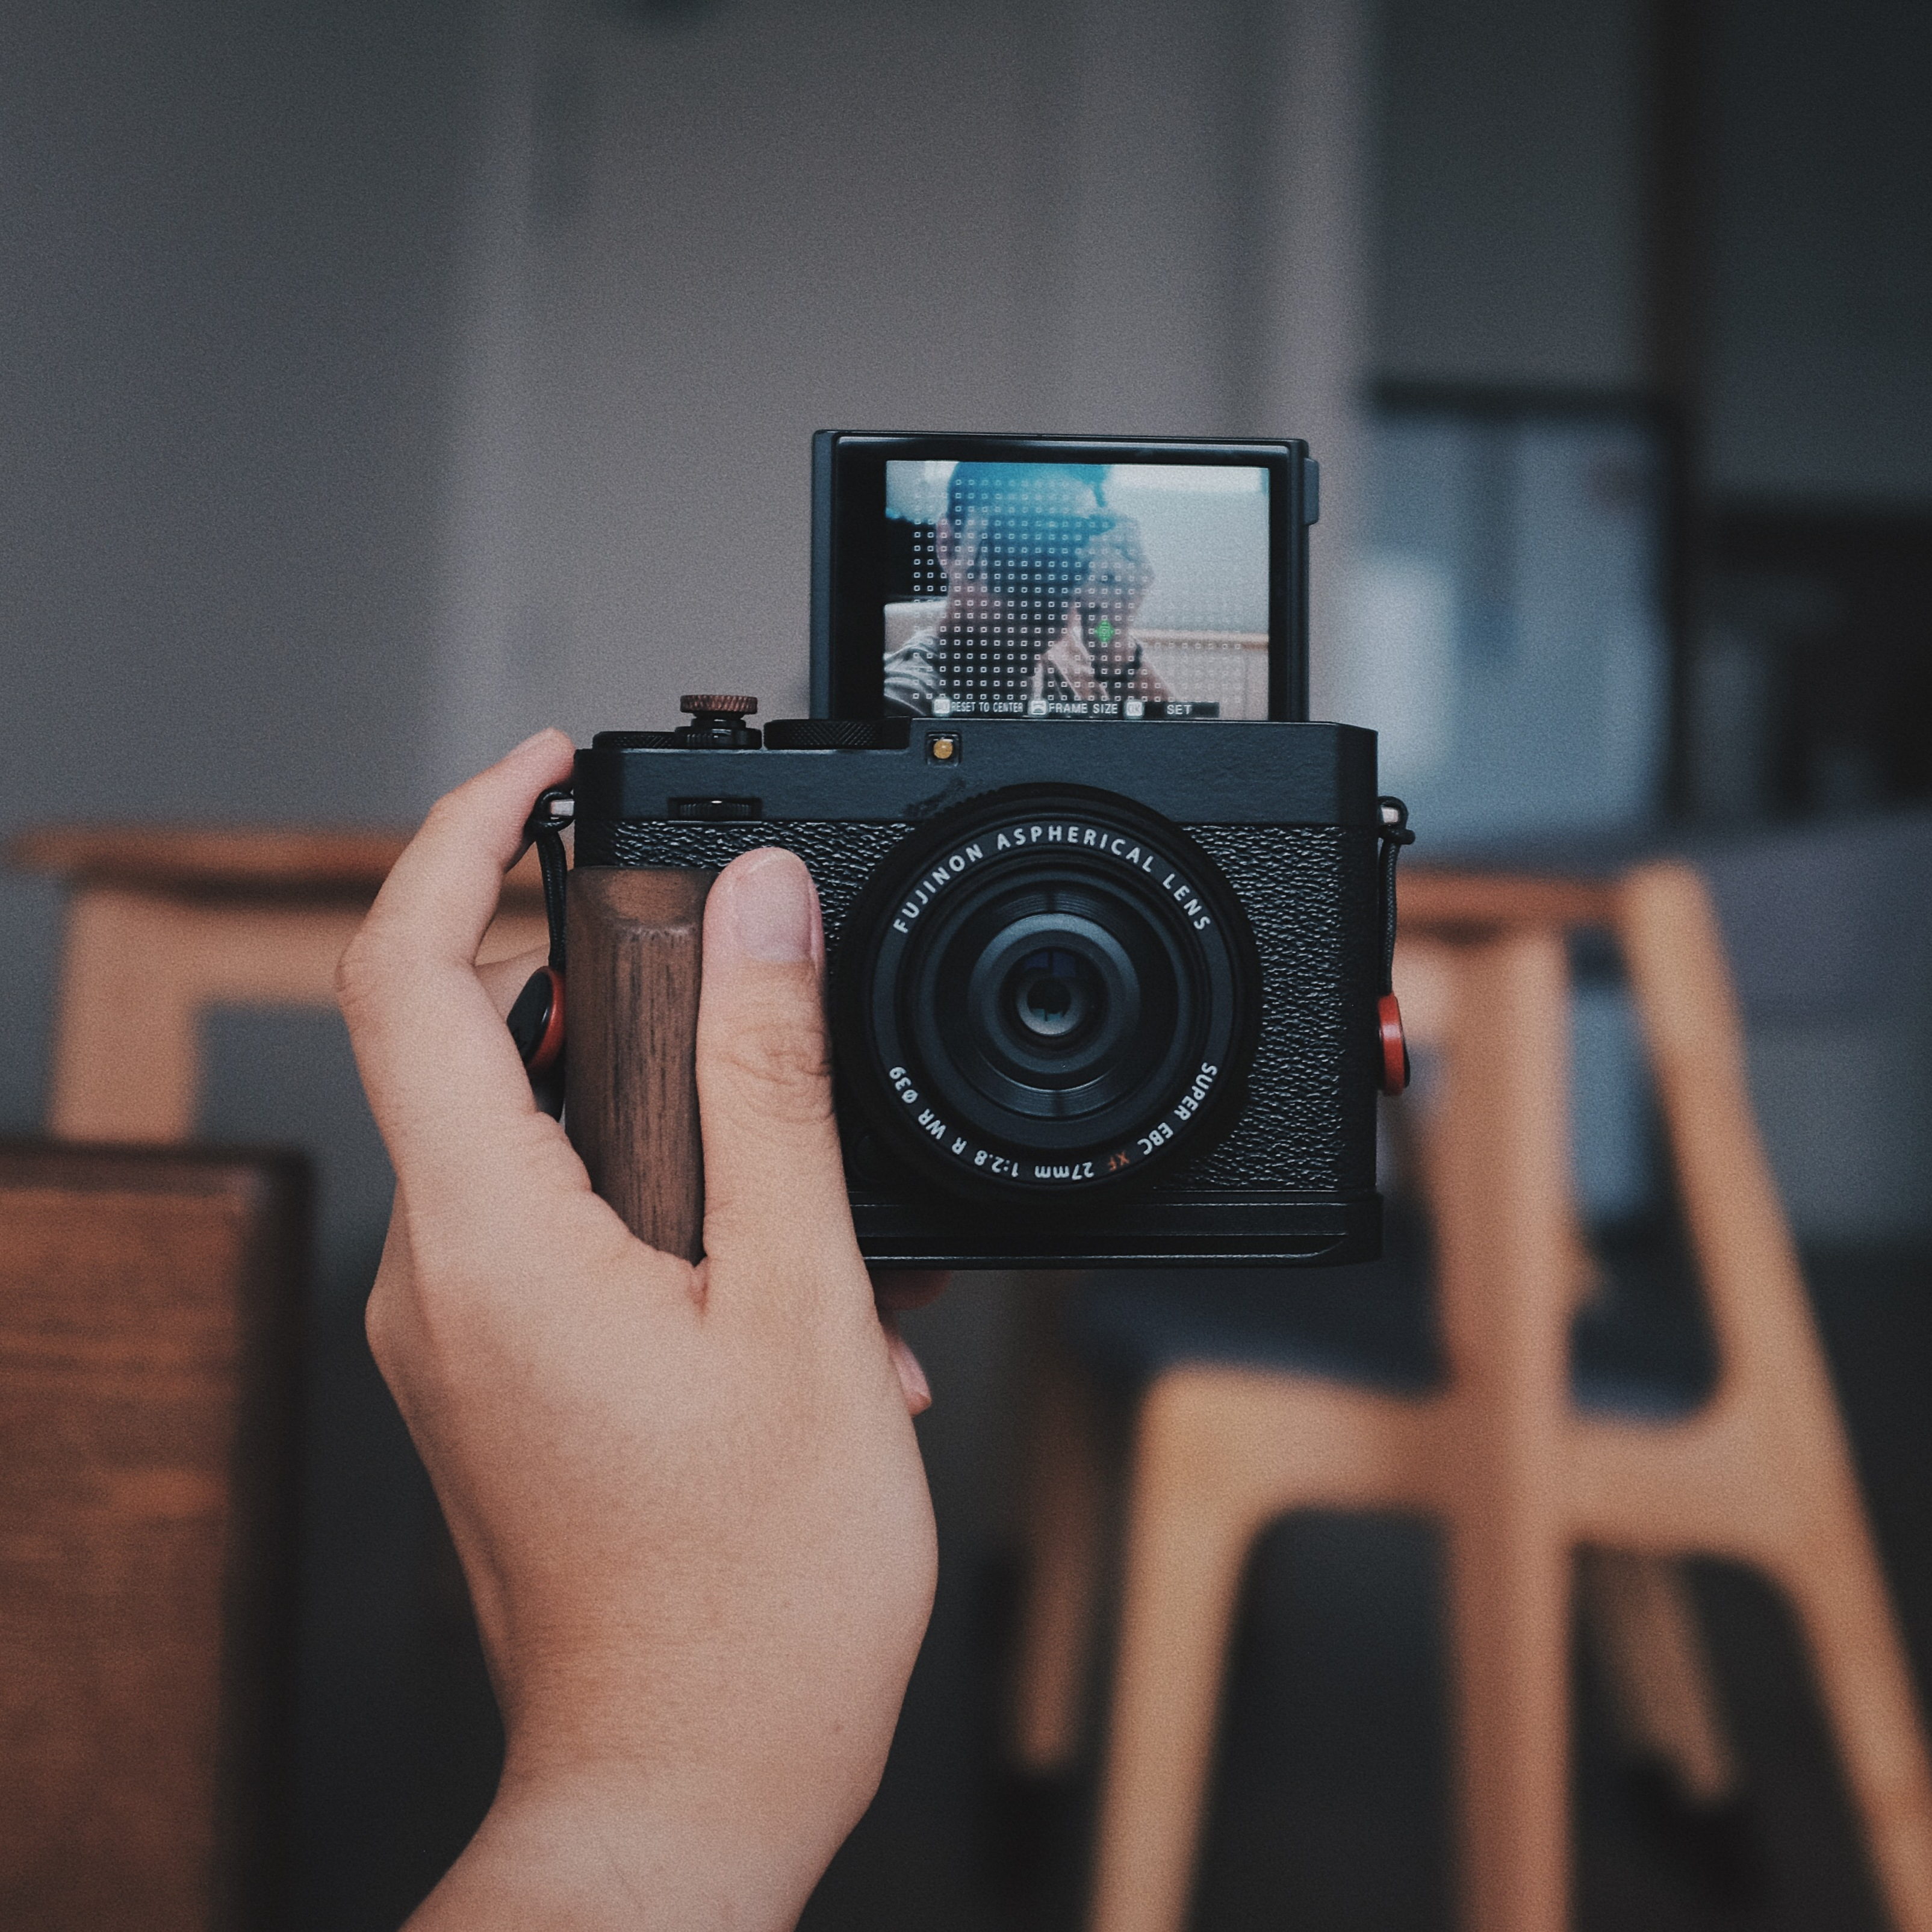
\includegraphics[width=\linewidth]{./today/coverpic.jpg}\par
        % \vskip 30pt
        \vfill

        \normalsize\upshape
        \copyright{} The Web Digest Project \hfill\large DATESTRING
    \end{center}
    % \vskip 20pt
    % \hrule
    % \vskip 10pt
    % \clearpage
}
\renewcommand{\contentsname}{\Huge\sffamily\bfseries Contents\par\vskip 20pt}
\newcounter{ipartcounter}
\setcounter{ipartcounter}{0}
\newcommand{\ipart}[1]{
    % \vskip 20pt
    \clearpage
    \stepcounter{ipartcounter}
    \phantomsection
    \addcontentsline{toc}{section}{#1}
    \begin{center}
        \Huge
        \sffamily\bfseries
        #1
    \end{center}
    \vskip 20pt
}
\newcommand{\entryitemHackernews}[3]{
    % argv: title, hnurl, rawurl
    \parbox{\linewidth}{
        \Large\rmfamily\bfseries#1\par\vskip 5pt
        \footnotesize\ttfamily\mdseries
        \href{#3}{#3}\par
        \textcolor{black!50}{\href{#2}{#2}}\par
    }\vskip 11pt
}
\newcommand{\entryitemGeneric}[2]{
    % argv: title, url
    \parbox{\linewidth}{
        \Large\rmfamily\bfseries#1\par\vskip 5pt
        \footnotesize\ttfamily\mdseries
        \href{#2}{#2}\par
    }\vskip 11pt
}






\begin{document}

\begin{titlepage}
	\makeheader
\end{titlepage}

\tableofcontents\clearpage


\ipart{Hacker News}
\entryitemTwoLinks{RealFill: Image completion using diffusion models}{https://news.ycombinator.com/item?id=37708292}{https://realfill.github.io/}

\entryitemTwoLinks{Homes ``unaffordable'' in 99\% of nation for average American}{https://news.ycombinator.com/item?id=37708109}{https://www.cbsnews.com/news/homes-for-sale-affordable-housing-prices/}

\entryitemTwoLinks{When CEOs Are Paid for Bad Performance (2005)}{https://news.ycombinator.com/item?id=37706876}{https://www.gsb.stanford.edu/insights/when-ceos-are-paid-bad-performance}

\entryitemTwoLinks{How a four-day workweek works, from the companies pulling it off}{https://news.ycombinator.com/item?id=37706596}{https://www.wsj.com/lifestyle/careers/how-a-4-day-workweek-actually-works-from-the-companies-pulling-it-off-1a5c0e2a}

\entryitemTwoLinks{Three Arrows Capital co-founder Zhu arrested in Singapore airport}{https://news.ycombinator.com/item?id=37705563}{https://techcrunch.com/2023/09/29/three-arrows-capital-co-founder-zhu-arrested-in-singapore-airport-sentenced-four-months-in-prison/}

\entryitemTwoLinks{Privacy washing: Google claims to support privacy while lobbying against it}{https://news.ycombinator.com/item?id=37705368}{https://proton.me/blog/google-lobbying}

\entryitemTwoLinks{Norway wants Facebook behavioral advertising banned across Europe}{https://news.ycombinator.com/item?id=37704859}{https://www.theregister.com/2023/09/29/norway\_facebook\_behavioral\_ads/}

\entryitemTwoLinks{Official U.S. government information about the Global Positioning System (GPS)}{https://news.ycombinator.com/item?id=37704593}{https://www.gps.gov/}

\entryitemTwoLinks{\$5k Google Jamboard dies in 2024–cloud-based apps will stop working, too}{https://news.ycombinator.com/item?id=37704537}{https://arstechnica.com/gadgets/2023/09/5000-google-jamboard-dies-in-2024-cloud-based-apps-will-stop-working-too/}

\entryitemTwoLinks{Encrypted Client Hello}{https://news.ycombinator.com/item?id=37703885}{https://blog.cloudflare.com/announcing-encrypted-client-hello/}

\entryitemTwoLinks{Senator Dianne Feinstein has died}{https://news.ycombinator.com/item?id=37703767}{https://www.bbc.com/news/world-us-canada-66963341}

\entryitemTwoLinks{Dianne Feinstein has died}{https://news.ycombinator.com/item?id=37703528}{https://www.nytimes.com/2023/09/29/us/politics/dianne-feinstein-dead-senate.html}

\entryitemTwoLinks{iPhone 15: users of Pro and Pro Max models complain of overheating issues}{https://news.ycombinator.com/item?id=37702846}{https://www.theguardian.com/technology/2023/sep/29/iphone-15-users-of-pro-and-pro-max-models-complain-of-overheating-issues}

\entryitemTwoLinks{Ask HN: Why isn't Phoenix/Elixir more mainstream?}{https://news.ycombinator.com/item?id=37702845}{https://news.ycombinator.com/item?id=37702845}

\entryitemTwoLinks{Everything authenticated by Microsoft is tainted}{https://news.ycombinator.com/item?id=37702095}{https://graz.social/@publicvoit/111147782761723981}

\entryitemTwoLinks{Leaked screenshot shows Amazon now tracking individual employee attendance}{https://news.ycombinator.com/item?id=37701222}{https://www.businessinsider.com/amazon-forced-rto-tracking-employee-office-attendance-2023-9}

\entryitemTwoLinks{Things Every Hacker Once Knew (2017)}{https://news.ycombinator.com/item?id=37701117}{http://www.catb.org/~esr/faqs/things-every-hacker-once-knew/}

\entryitemTwoLinks{Burning money on paid ads for a dev tool – what we've learned}{https://news.ycombinator.com/item?id=37700847}{https://posthog.com/blog/dev-marketing-paid-ads}

\entryitemTwoLinks{Richard Stallman reveals he has cancer in the GNU 40 Hacker Meeting talk [video]}{https://news.ycombinator.com/item?id=37699851}{https://audio-video.gnu.org/video/gnu40/rms-gnu40.webm}

\entryitemTwoLinks{Costco gold bars are selling out within hours}{https://news.ycombinator.com/item?id=37699396}{https://www.cnbc.com/2023/09/27/costco-is-selling-gold-bars-and-they-are-selling-out-within-a-few-hours.html}

\ipart{V2EX}
\entryitemGeneric{\hskip 0pt{}[问与答] 假如身边同事说以前拍过 A 片,你对他/她会是什么感觉?}{https://www.v2ex.com/t/945394}

\entryitemGeneric{\hskip 0pt{}[Apple] 纵观 618 手机推荐,好像 iphone15 的最大讨论是 C 口?}{https://www.v2ex.com/t/945393}

\entryitemGeneric{\hskip 0pt{}[问与答] 配一台 PVE 专用主机}{https://www.v2ex.com/t/945392}

\entryitemGeneric{\hskip 0pt{}[问与答] 请教一下,我这老古董的电脑配置,可以更新下显卡么?谢谢 V 友。}{https://www.v2ex.com/t/945391}

\entryitemGeneric{\hskip 0pt{}[程序员] 很多程序员确实会被后浪拍死在沙滩上}{https://www.v2ex.com/t/945390}

\entryitemGeneric{\hskip 0pt{}[推广] 手机版 ChatGPT,不需要魔法上网}{https://www.v2ex.com/t/945389}

\entryitemGeneric{\hskip 0pt{}[NAS] Nas 用作备份还是主存储}{https://www.v2ex.com/t/945387}

\entryitemGeneric{\hskip 0pt{}[问与答] virtctl 上传一个 iso 文件报错求助}{https://www.v2ex.com/t/945386}

\entryitemGeneric{\hskip 0pt{}[iDev] 看了微软的 documentation 才知道 macCatalyst 的预设 idiom 真的就是 .pad。}{https://www.v2ex.com/t/945385}

\entryitemGeneric{\hskip 0pt{}[程序员] 2 个适合做 AI 项目的域名}{https://www.v2ex.com/t/945384}

\entryitemGeneric{\hskip 0pt{}[Markdown] 贺 WWDC 😀,促销一下我的 App,时间 6/3~6/10,共 7 天,最低 6 折!}{https://www.v2ex.com/t/945383}

\entryitemGeneric{\hskip 0pt{}[OpenAI] depay 被 gpt 禁用了,大家有别的支付方式吗?}{https://www.v2ex.com/t/945382}

\entryitemGeneric{\hskip 0pt{}[分享发现] 去广告的油猴脚本里偷偷藏了个广告 dadiyouhui}{https://www.v2ex.com/t/945379}

\entryitemGeneric{\hskip 0pt{}[Flutter] 求助 flutter 代码 按钮提示音 问题}{https://www.v2ex.com/t/945377}

\entryitemGeneric{\hskip 0pt{}[生活] 失业设计师推广一下自创品牌香薰}{https://www.v2ex.com/t/945375}

\entryitemGeneric{\hskip 0pt{}[问与答] 美国 non tax resident  alien 个税 收入来自 paypal}{https://www.v2ex.com/t/945374}

\entryitemGeneric{\hskip 0pt{}[程序员] 计划写个全栈的浏览器插件开发教程,内容涉及 Web3, 前端,后端,浏览器开发,有没有感兴趣的!}{https://www.v2ex.com/t/945373}

\entryitemGeneric{\hskip 0pt{}[问与答] 我常常固执地沉浸在负面情绪中}{https://www.v2ex.com/t/945372}

\entryitemGeneric{\hskip 0pt{}[程序员] 程序员的悲哀是什么[转]}{https://www.v2ex.com/t/945371}

\entryitemGeneric{\hskip 0pt{}[北京] 谁有推荐配眼镜的地方}{https://www.v2ex.com/t/945366}

\entryitemGeneric{\hskip 0pt{}[问与答] Win10 自动安装管家}{https://www.v2ex.com/t/945365}

\entryitemGeneric{\hskip 0pt{}[iPhone] iPhone 第三方无线充电器推荐}{https://www.v2ex.com/t/945363}

\entryitemGeneric{\hskip 0pt{}[上海] 房东直租静安区二房无中介费}{https://www.v2ex.com/t/945362}

\entryitemGeneric{\hskip 0pt{}[问与答] s23u 港版}{https://www.v2ex.com/t/945361}

\entryitemGeneric{\hskip 0pt{}[硬件] 第一次攒机, NAS + HPC 求建议}{https://www.v2ex.com/t/945360}

\entryitemGeneric{\hskip 0pt{}[问与答] 打算在理想 L9 后排看奈飞,买了谷歌 TV,求推荐能装 CLASH 插件的 USB 无线 4G 网卡}{https://www.v2ex.com/t/945359}

\entryitemGeneric{\hskip 0pt{}[问与答] GitHub 改用户名,会对已有 repository 造成啥影响吗?}{https://www.v2ex.com/t/945357}

\entryitemGeneric{\hskip 0pt{}[深圳] 人在深圳,卖家电啦, TCL 家电,内购价,有需要购买家电的可以找我,提供贴心服务,优惠大大滴,全部都是成本价,不赚家人们一分钱,只为完成 kpi}{https://www.v2ex.com/t/945356}

\entryitemGeneric{\hskip 0pt{}[问与答] win10 睡眠唤醒之后,键盘无法用。}{https://www.v2ex.com/t/945355}

\entryitemGeneric{\hskip 0pt{}[问与答] 咨询一下大佬们,四个风扇的乔思伯 D41 Mesh 网孔版 白色,该怎么安排风道?}{https://www.v2ex.com/t/945354}

\entryitemGeneric{\hskip 0pt{}[奇思妙想] 在无 KVM 功能但有一线通的显示器上把它变成手动 KVM 模式是否可行?}{https://www.v2ex.com/t/945353}

\entryitemGeneric{\hskip 0pt{}[问与答] bilibili 电视 app 除了原生还有什么选择吗}{https://www.v2ex.com/t/945352}

\entryitemGeneric{\hskip 0pt{}[Apple] 总觉得 MBP 比 mac studio 用起来流畅的多。}{https://www.v2ex.com/t/945351}

\entryitemGeneric{\hskip 0pt{}[程序员] 大家觉得现在 CS Research 还有什么领域不卷}{https://www.v2ex.com/t/945350}

\entryitemGeneric{\hskip 0pt{}[Surge] [Surge for Mac 5 ] 160RMB/位}{https://www.v2ex.com/t/945349}

\entryitemGeneric{\hskip 0pt{}[生活] 查出了不能生育,心里郁闷}{https://www.v2ex.com/t/945348}

\entryitemGeneric{\hskip 0pt{}[分享创造] 面试工具 InterviewAI 在 ProductHunt 上发布啦}{https://www.v2ex.com/t/945347}

\entryitemGeneric{\hskip 0pt{}[Docker] docker run 成功, docker compose up 失败?}{https://www.v2ex.com/t/945345}

\entryitemGeneric{\hskip 0pt{}[分享发现] 看在 CPU 的面子上,多多入手红米 NOTE12 Turbo}{https://www.v2ex.com/t/945344}

\entryitemGeneric{\hskip 0pt{}[Amazon Web Services] AWS 的 cloudwatch 是必须使用的吗?}{https://www.v2ex.com/t/945343}

\entryitemGeneric{\hskip 0pt{}[问与答] 有没有卸载 Anaconda 不影响已经配置的环境切换到 Miniconda 的办法?}{https://www.v2ex.com/t/945341}

\entryitemGeneric{\hskip 0pt{}[分享创造] 低成本做个 ChatGPT 聊天机器人}{https://www.v2ex.com/t/945340}

\entryitemGeneric{\hskip 0pt{}[问与答] 海南的国企,海南征信,中科电海信院有没有好的建议}{https://www.v2ex.com/t/945338}

\entryitemGeneric{\hskip 0pt{}[生活] 如何处理收废品的大喇叭扰民?}{https://www.v2ex.com/t/945337}

\entryitemGeneric{\hskip 0pt{}[问与答] 二手车混动求推荐贬值超快的}{https://www.v2ex.com/t/945336}

\entryitemGeneric{\hskip 0pt{}[YubiKey] 收购两只 yubikey 5 nfc}{https://www.v2ex.com/t/945335}

\entryitemGeneric{\hskip 0pt{}[问与答] 除了豆瓣网,还有什么中文的图书、书评网吗?}{https://www.v2ex.com/t/945334}

\entryitemGeneric{\hskip 0pt{}[问与答] 高价求各种引流大佬}{https://www.v2ex.com/t/945332}

\entryitemGeneric{\hskip 0pt{}[OpenAI] 4.0api,claude 100kapi}{https://www.v2ex.com/t/945329}

\entryitemGeneric{\hskip 0pt{}[问与答] 求问 hw-v2-web-player-tracker.biliapi 是干什么的, clash 速率离奇达到 300MB/s}{https://www.v2ex.com/t/945326}

\ipart{Solidot}
\entryitemGeneric{\hskip 0pt{}科学家首次计算出恒星周围的含水量}{https://www.solidot.org/story?sid=77506}

\entryitemGeneric{\hskip 0pt{}印度要求发布模型需得到政府批准}{https://www.solidot.org/story?sid=77505}

\entryitemGeneric{\hskip 0pt{}防火墙泄漏跨国流量}{https://www.solidot.org/story?sid=77504}

\entryitemGeneric{\hskip 0pt{}中国盗版动漫网站主犯被判三年缓刑三年六个月}{https://www.solidot.org/story?sid=77503}

\entryitemGeneric{\hskip 0pt{}《ACM 通讯》正式拥抱开放获取}{https://www.solidot.org/story?sid=77502}

\entryitemGeneric{\hskip 0pt{}Linux 基金会的新项目得到了盖茨基金会的资助}{https://www.solidot.org/story?sid=77501}

\entryitemGeneric{\hskip 0pt{}Mozilla 的 Firefox 和谋智的火狐}{https://www.solidot.org/story?sid=77500}

\entryitemGeneric{\hskip 0pt{}两部星战电影准备开拍}{https://www.solidot.org/story?sid=77499}

\entryitemGeneric{\hskip 0pt{}全球人口的八分之一肥胖}{https://www.solidot.org/story?sid=77498}

\entryitemGeneric{\hskip 0pt{}Google 解雇了组建工会的 YouTube 合同工}{https://www.solidot.org/story?sid=77497}

\entryitemGeneric{\hskip 0pt{}座头鲸首次观察到同性性交}{https://www.solidot.org/story?sid=77496}

\entryitemGeneric{\hskip 0pt{}微软撤下导致``内存不足''错误的 Edge 更新}{https://www.solidot.org/story?sid=77495}

\entryitemGeneric{\hskip 0pt{}马斯克起诉 OpenAI 和 Sam Altman``违反合同''}{https://www.solidot.org/story?sid=77494}

\entryitemGeneric{\hskip 0pt{}美国疾控中心称 COVID-19 越来越像流感}{https://www.solidot.org/story?sid=77493}

\entryitemGeneric{\hskip 0pt{}BCUninstaller:轻松卸载你不想要的应用}{https://www.solidot.org/story?sid=77492}

\ipart{联合早报}
\entryitemWithDescription{杨丹旭:中国股民能否过个安心年?}{https://www.zaobao.com/news/china/story20240207-1466809}{``人生不仅仅只有股市,还有父母、爱人、孩子和朋友,建议投资者可以暂时离开股市,放下执念,给自己换一个心情,以轻松平和的心情迎接新年的到来。'' 中国股市近期哀鸿遍野,面对吐槽与质疑,一家中国上市公司上周五(2月2日)在互动平台上如此劝喻投资者。 这家公司还安抚股民:``对于这个市场的波动,一个公司很难改变什么,个人投资者也很难改变,我们只能接受和适应这个市场环境……}

\entryitemWithDescription{台中市爆台糖肉品含瘦肉精 检验结果星期三揭晓}{https://www.zaobao.com/news/china/story20240206-1466794}{台中市政府抽验年节肉品,发现台糖安心豚冷冻梅花肉片,含有不得验出的瘦肉精``西布特罗''。(香港中通社) 农历新年将届,台中市政府启动大规模食品安全抽查,从公营事业台糖公司梅花肉片检出含有禁用的瘦肉精``西布特罗''(Cimbuterol)。但台湾政府强调,同批肉品样品的瘦肉精零检出。双方双轨复验结果,可望于星期三(2月7日)出炉……}

\entryitemWithDescription{中国粉丝办观影派对盼泰勒丝赴华演出 政治因素或成阻碍}{https://www.zaobao.com/news/china/story20240206-1466790}{手持荧光棒、身着闪亮连衣裙、佩戴友谊手环,美国歌坛天后泰勒丝的中国粉丝将原本安静的电影院变成了他们偶像的派对现场。图为2024年2月3日,泰勒丝的中国歌迷在北京一家电影院观看演唱会电影《泰勒丝:时代巡回演唱会》。(法新社) (北京法新电)美国歌坛天后泰勒丝(Taylor Swift)的中国粉丝们在电影院举办观影派对盼她赴华演出,但有人担忧她的政治立场会成为阻碍……}

\entryitemWithDescription{香港表演赛梅西未上场:建制阵营质疑背后有外部势力破坏}{https://www.zaobao.com/news/china/story20240206-1466787}{热情的梅西粉丝2月4日在香港表演赛开场前,兴高采烈地在观众席上举牌以西班牙文向偶像喊话:``可以给我你的球衣吗?''料想不到的是,梅西最后并未下场。(法新社) 美国足球大联盟球会迈阿密国际(Inter Miami)访问香港的表演赛,由于球王梅西未上场,点燃全城球迷怒火,建制派阵营更质疑梅西是否背后受压而不出场,担心日后香港会面对新的破坏行动。不过,有受访学者认为这些看法流于阴谋论……}

\entryitemWithDescription{中国遭遇大范围强雨雪天气 春运返乡路受阻}{https://www.zaobao.com/news/china/story20240206-1466775}{(北京/上海综合讯)中国中东部地区本月以来持续出现低温雨雪冰冻天气,令民众的春节返乡路变得更为复杂与艰难。在中部省份湖北,高速公路出现大范围拥堵现象,有车主被困三天三夜无法动弹。 综合央视网与第一财经网报道,自1月31日开始,冰冻雨雪天气席卷中国中东部,多地遭遇了2009年以来冬季最强雨雪冰冻天气……}

\entryitemWithDescription{澳籍华裔作家杨恒均被判死缓 阿尔巴尼斯表达愤慨}{https://www.zaobao.com/news/china/story20240206-1466766}{澳洲总理阿尔巴尼斯星期二(2月6日)在堪培拉受访时,对澳籍华裔作家杨恒均被判死缓表达愤慨。图为阿尔巴尼斯1月25日在堪培拉的全国媒体俱乐部发言。(彭博社) (悉尼综合电)澳大利亚总理阿尔巴尼斯对澳籍华裔作家杨恒均被判死缓表达愤慨,并誓言将持续争取让他获释……}

\entryitemWithDescription{香港机场男工遭飞机碾压死亡}{https://www.zaobao.com/news/china/story20240206-1466760}{(香港综合讯)香港国际机场星期二(2月6日)凌晨发生一起离奇的意外事故,一名飞机拖车人员疑似遭飞机辗压致死。 综合《星岛日报》《明报》、大公文汇全媒体报道,死者为一名34岁的非华裔男子,持有香港身份证,是一名负责将飞机拖出跑道的工作人员。他星期二凌晨与另一名负责驾驶拖飞机拖车的60岁男子,将一架飞机拖至西停机坪……}

\entryitemWithDescription{香港演艺学院叫停毕业生无政府题材作品}{https://www.zaobao.com/news/china/story20240206-1466746}{(香港综合讯)香港演艺学院舞台剧毕业作品《一个无政府主义者的意外死亡》原定下星期六(2月17日)上演,但被校方临时取消。 综合《星岛日报》与端传媒报道,香港演艺学院应届毕业生筹备的上述剧目,在学院网站的剧目资讯突然下架。官网星期一(2月5日)公告称,``由于学院制作安排之变动'',该剧演出将会取消。校方在回复港媒询问时,没有交代详细原因……}

\entryitemWithDescription{危地马拉考虑与中国大陆发展贸易 但维持与台湾关系}{https://www.zaobao.com/news/china/story20240206-1466745}{危地马拉外交部长马丁内斯当地时间星期一(2月5日)接受路透社访问时说,该国考虑与中国大陆开展正式贸易关系,但计划与台湾维持现有的外交关系。(路透社) (危地马拉城综合讯)危地马拉外交部长马丁内斯说,该国考虑与中国大陆开展正式贸易关系,但计划维持与台湾现有的外交关系。 马丁内斯星期一(2月5日)告诉路透社,``我们将继续与台湾保持一贯的合作关系……}

\entryitemWithDescription{戴庆成:香港盛事经济能奏效么?}{https://www.zaobao.com/news/china/story20240206-1466585}{阿根廷球王梅西(右一)领军的美职联球队国际迈阿密星期日(2月4日)在香港大球场和香港队进行表演赛,但他全场只坐在场边看球,令球迷极度失望。(彭博社) 香港足球迷最近的心情应该很亢奋,除了因为港队在亚洲杯表现不俗,以及在今年省港杯首回合赛事先拔头筹打败广东队,另一个更重要的原因是阿根廷球王梅西时隔近10年重临香港……}

\entryitemWithDescription{台湾立法院龙头之战 延烧出民进党不同派系的新阁揆卡位战}{https://www.zaobao.com/news/china/story20240206-1466594}{台湾立法院龙头之战,延烧出民进党内部不同派系的新阁揆卡位战。 在野民众党(白)称,立法院龙头之争``电话门''事件是执政的民进党(绿)内斗,民众党被牵扯其中,为此在星期一(2月5日)对民进党发言人吴铮等相关人士和媒体一并提起民事告诉。民进党也回应,乐于到法院还原事实真相……}

\entryitemWithDescription{澳洲华裔作家杨恒均被判死缓 分析:将成为中澳新冲突点}{https://www.zaobao.com/news/china/story20240205-1466589}{澳大利亚华裔作家杨恒均星期一(2月5日)被北京法院判处死刑缓期执行。(杨恒均X平台(前称推特)账号) 在中国被控间谍罪、已经被关押长达五年的澳大利亚华裔作家杨恒均,星期一(2月5日)被北京法院判处死刑缓期执行,预计两年后减为无期徒刑。 学者研判,杨恒均事件将成为中澳之间的一个新冲突点,可能进一步扰动地缘政治,甚至加速澳英美三方安全伙伴关系(AUKUS)扩大阵容……}

\entryitemWithDescription{传美日军演首将中国列假想敌 模拟应对台海危机}{https://www.zaobao.com/news/china/story20240205-1466574}{(东京综合讯)据日媒报道,美国和日本在联合指挥所演习中,首次将中国列为假想敌,凸显围绕台海地缘政治紧张局势正日益加剧。不过据美媒报道,日本防卫省否认了这一消息。 日本共同社星期天(2月4日)引述多位政府相关人士透露,日本自卫队和美军在进行中的最高级别演习,与以往使用虚构名称不同,这次直接指定中国为虚拟敌国。 这次演习于2月1日开始,预计将持续至2月8日。演习采用计算机模拟,并以台海危机为主要情境……}

\entryitemWithDescription{中国报告JN.1变异株流行 春节期间冠病疫情有上升风险}{https://www.zaobao.com/news/china/story20240205-1466553}{(北京综合讯)中国疾病预防控制中心通报,冠病变异株JN.1已成为中国本土的优势流行株,由于春节期间的人口流动和聚集,预计疫情将逐步上升。 综合人民网、澎湃新闻等报道,中国疾控中心病毒病预防控制所研究员陈操星期日(2月4日)在国家卫生健康委员会新闻发布会上说,尽管目前中国冠病疫情仍呈低水平流行,但近期病例报告和哨点医院检测阳性率等指标显示出小幅增加,提示冠病疫情呈现上升趋势……}

\entryitemWithDescription{中俄就人工智能的军事使用磋商协调}{https://www.zaobao.com/news/china/story20240205-1466548}{(北京综合讯)中国和俄罗斯已同意就人工智能的军事使用进行磋商和协调,这项技术正在成为北京与华盛顿竞争的新战线。 《南华早报》报道,俄罗斯外交部上星期五(2月2日)在声明中说,俄中部门官员上星期四(2月1日)在北京举行的会谈中,针对将人工智能技术用于军事目的进行了``详细的评估交流''……}

\entryitemWithDescription{美军长驻台湾陆军两栖营 助台军学用微型无人机}{https://www.zaobao.com/news/china/story20240205-1466543}{美国陆军特种部队今年起将派顾问长驻台湾陆军两栖营。图为台湾军人1月31日在台东一个军事基地进行演习。(路透社) (台北/华盛顿综合讯)绰号``绿扁帽''的美国陆军特种部队今年起将派顾问长驻台湾陆军两栖营,主要协助台特战部队学习使用微型无人机等……}

\entryitemWithDescription{港府对梅西表演赛未上场``极度失望'' 主办方撤回资助申请}{https://www.zaobao.com/news/china/story20240205-1466540}{迈阿密国际队星期日(2月4日)在香港进行季前友谊赛,但该队的阿根廷足球巨星梅西全程坐在后备席未上场。全场球迷表达不满,大喊要求退钱。(法新社) (香港综合讯)美国足球大联盟球会迈阿密国际(Inter Miami)星期天在香港举行表演赛,球星梅西因肌肉炎症未上场比赛,令众多球迷大感不满。港府两度发声对梅西未能出赛表示极度失望,赛事主办方也宣布撤回赞助款项申请……}

\entryitemWithDescription{中国疫后入境旅游恢复缓慢}{https://www.zaobao.com/news/china/story20240205-1466522}{报告显示,中国去年外国人出入境次数仅恢复到冠病疫情暴发前的36\%。图为北京首都机场的一名旅客在查看机场出发信息指示牌。(彭博社) (北京综合讯)官方研究机构公布的报告显示,中国去年外国人出入境次数仅恢复到冠病疫情暴发前的36\%。 根据中国文化和旅游部旗下的专业研究机构中国旅游研究院微信公众号消息,上述数据来自该院2月1日发布的《中国入境旅游发展报告(2023-2024)》……}

\entryitemWithDescription{于泽远:半年12名将军落马}{https://www.zaobao.com/news/china/story20240205-1466355}{中国全国人大官网近日发布2024年第一号《全国人大常委会公报》,首次披露了去年12月下旬被宣布罢免全国人大代表职务的九名军方高级将领的职位、原因和时间。他们全都涉嫌``严重违纪违法''。 这九名将领包括三名上将、四名中将,两名少将……}

\entryitemWithDescription{港府考虑23条立法延迟或阻止嫌疑人见律师 防通风报信}{https://www.zaobao.com/news/china/story20240204-1466382}{(香港综合讯)香港特区政府正就《基本法》第23条立法咨询公众,其中考虑延长被捕者的最长拘留期。港府或借鉴英国做法,允许警司阻止被捕者咨询特定律师,以防止信息泄露和危害国家安全的行为,并倾向由司法机关负责批核这一过程。 综合《明报》、Now新闻等报道,《基本法》第23条立法咨询中一个关键议题,是考虑延长被捕者最多48小时羁押期限……}

\entryitemWithDescription{腾讯去年解聘120多名涉舞弊和贪腐员工}{https://www.zaobao.com/news/china/story20240204-1466381}{腾讯去年解聘120多名违反公司的反舞弊规定的员工。(路透社) (北京综合讯)中国互联网巨头腾讯去年解聘120多名违反公司的反舞弊规定的员工,其中包括涉贪和腐败行为。 腾讯反舞弊调查部星期五(2月2日)在官方微信公号上通报,2023年全年,共发现并查处触犯``腾讯高压线''案件70余起,120余人因触犯``腾讯高压线''被解聘,近20人因涉嫌犯罪被移送公安机关处理……}

\entryitemWithDescription{春节猪肉消费下降 引发通缩担忧}{https://www.zaobao.com/news/china/story20240204-1466374}{中国居民消费价格指数(CPI)去年12月已连续三个月出现下降,且这种趋势或持续至今年。食品占CPI约五分之一,猪肉又是重要组成部分。图为1月17日,福建福州的市民在超市购买猪肉。(中新社) (北京彭博电)春节作为中国重要节日,传统上家家户户会买猪肉烹制各式菜肴,猪肉需求也往往较高。但据美媒报道,尽管今年春节猪肉价格下降,民众对猪肉的兴趣却明显减少,加剧了中国经济通缩的担忧……}

\ipart{Dribbble}
\entryitemGeneric{\hskip 0pt{}Shiner Gin}{https://dribbble.com/shots/23291265}

\entryitemGeneric{\hskip 0pt{}𝐓𝐡𝐞 𝐑𝐞-𝐆𝐢𝐟𝐭𝐞𝐫}{https://dribbble.com/shots/23283456}

\entryitemGeneric{\hskip 0pt{}Goodies Ice House}{https://dribbble.com/shots/23282437}

\entryitemGeneric{\hskip 0pt{}2023 Recap}{https://dribbble.com/shots/23282303}

\entryitemGeneric{\hskip 0pt{}Rebel Wear}{https://dribbble.com/shots/23256082}

\entryitemGeneric{\hskip 0pt{}Playful Paws at Work}{https://dribbble.com/shots/23281289}

\entryitemGeneric{\hskip 0pt{}Logo and mascot for "Houblo"}{https://dribbble.com/shots/23280500}

\entryitemGeneric{\hskip 0pt{}The Scent of Seasonal Dread🕯️🎄}{https://dribbble.com/shots/23282168}

\entryitemGeneric{\hskip 0pt{}Jason Broyles}{https://dribbble.com/shots/23143895}

\entryitemGeneric{\hskip 0pt{}Residential WIP}{https://dribbble.com/shots/23281779}

\entryitemGeneric{\hskip 0pt{}Tarot card \#02: The High Priestess}{https://dribbble.com/shots/23283002}

\entryitemGeneric{\hskip 0pt{}olives}{https://dribbble.com/shots/23274110}

\entryitemGeneric{\hskip 0pt{}Drijfkracht}{https://dribbble.com/shots/23272957}

\entryitemGeneric{\hskip 0pt{}Nightweaver Book}{https://dribbble.com/shots/23272131}

\entryitemGeneric{\hskip 0pt{}Squirtle, Bulbasaur \& Charmander}{https://dribbble.com/shots/23274016}

\entryitemGeneric{\hskip 0pt{}"Slay?" … "Sleigh."}{https://dribbble.com/shots/23241933}

\entryitemGeneric{\hskip 0pt{}Wonka x theory11 Playing Cards}{https://dribbble.com/shots/23259494}

\entryitemGeneric{\hskip 0pt{}Yosemite National Park}{https://dribbble.com/shots/23258567}

\entryitemGeneric{\hskip 0pt{}COP28}{https://dribbble.com/shots/23180619}

\entryitemGeneric{\hskip 0pt{}Glyph Beer 16}{https://dribbble.com/shots/23258745}

\entryitemGeneric{\hskip 0pt{}Manufactory}{https://dribbble.com/shots/23258744}

\entryitemGeneric{\hskip 0pt{}Jobsity Industries}{https://dribbble.com/shots/22760054}

\entryitemGeneric{\hskip 0pt{}Case Study: Advocacy Through Walls Website}{https://dribbble.com/shots/23258899}

\entryitemGeneric{\hskip 0pt{}Time Machine 64}{https://dribbble.com/shots/23258616}





\clearpage
\leavevmode\vfill
\footnotesize

Copyright \copyright{} DATESTRING Neruthes and other contributors.

The entries listed in this newsletter may be copyrighted by their respective creators.

This newsletter is generated by the Web Digest project.

Newsletters are also delivered via Telegram channel\\
\CJKunderline{\href{https://t.me/webdigestchannel}{t.me/webdigestchannel}}.

This newsletter is available in PDF format at\\
\CJKunderline{\href{https://webdigest.pages.dev/}{webdigest.pages.dev}}.

The source code being used to generated this newsletter is available at\\
\CJKunderline{\href{https://github.com/neruthes/webdigest/}{github.com/neruthes/webdigest}}.


\coverpic{https://unsplash.com/photos/an-aerial-view-of-a-beach-with-trees-in-the-background-ciYs2jFPqJ4}{Aditya Chinchure}


\end{document}
